%                                                                 aa.dem
% AA vers. 8.2, LaTeX class for Astronomy & Astrophysics
% demonstration file
%                                                       (c) EDP Sciences
%-----------------------------------------------------------------------
%
%\documentclass[referee]{aa} % for a referee version
%\documentclass[onecolumn]{aa} % for a paper on 1 column  
%\documentclass[longauth]{aa} % for the long lists of affiliations 
%\documentclass[rnote]{aa} % for the research notes
%\documentclass[letter]{aa} % for the letters 
%\documentclass[bibyear]{aa} % if the references are not structured 
% according to the author-year natbib style

%
\documentclass{aa}  

%
\usepackage{graphicx}
%%%%%%%%%%%%%%%%%%%%%%%%%%%%%%%%%%%%%%%%
\usepackage{txfonts}
%%%%%%%%%%%%%%%%%%%%%%%%%%%%%%%%%%%%%%%%
\usepackage{hyperref}
% To add links in your PDF file, use the package "hyperref"
% with options according to your LaTeX or PDFLaTeX drivers.
%
%\usepackage{url}
%\usepackage{fontawesome}

%\usepackage{xspace}
%\usepackage{subcaption}

\def\detJ{\mathrm{det}J}

\def\tein{\theta_{\mathrm{Ein}}}
\def\trad{\theta_{\mathrm{rad}}}
\def\tsis{\theta_{\mathrm{Ein}}^{\mathrm{(SIS)}}}
\def\meantsis{<\tsis>}
\def\stdtsis{\sigma(\tsis)}

\def\teinein{\theta_{\mathrm{Ein}}^*}
\def\betaein{\beta^*}

\def\toneobs{\theta_1^{\mathrm{obs}}}
\def\ttwoobs{\theta_2^{\mathrm{obs}}}

\def\moneobs{m_1^{\mathrm{obs}}}
\def\mtwoobs{m_2^{\mathrm{obs}}}

\def\asymm{\xi_{\mathrm{asymm}}}
\def\rmur{r_{\mu_r}}
\def\rmurobs{r_{\mu_r}^{(\mathrm{obs})}}
\def\mumin{\mu_{\mathrm{min}}}
\def\betamax{\beta_{\mathrm{max}}}
\def\betasl{\beta_{\mathrm{SL}}}

\def\hyperpars{\boldsymbol{\eta}}
\def\indpar{\boldsymbol{\psi}}
\def\indpari{\boldsymbol{\psi}_i}

\def\nsource{N_{\mathrm{s}}}
\def\nbkg{n_{\mathrm{bkg}}}

\def\psilens{\boldsymbol{\psi}_\mathrm{g}}
\def\psisource{\boldsymbol{\psi}_\mathrm{s}}
\def\psisourcetwo{\boldsymbol{\psi}_{\mathrm{s},2}}
\def\psisourcens{\boldsymbol{\psi}_{\mathrm{s},\nsource}}
\def\psisourcenobeta{\boldsymbol{\psi}_\mathrm{s}^{(-\boldsymbol\beta)}}

\def\Nlens{N_{\mathrm{lens}}}
\def\Nnot{N_{\mathrm{not}}}

\def\prlens{{\rm P}_\mathrm{g}}
\def\prsource{{\rm P}_\mathrm{s}}
\def\prlensone{{\rm P}_{\mathrm{g},1}}
\def\prlenstwo{{\rm P}_{\mathrm{g},2}}
\def\prsourceone{{\rm P}_{\mathrm{s},1}}
\def\prsourcetwo{{\rm P}_{\mathrm{s},2}}
\def\prsl{{\rm P}_\mathrm{{SL}}}
\def\prslone{{\rm P}_{\mathrm{SL},1}}
\def\prsltwo{{\rm P}_{\mathrm{SL},2}}

\def\prsourcenobeta{{\rm P}_\mathrm{s}^{(-\boldsymbol\beta)}}

\def\pdet{{\rm P}_\mathrm{det}}
\def\pdetone{{\rm P}_{\mathrm{det},1}}
\def\pdettwo{{\rm P}_{\mathrm{det},2}}
\def\crosssect{\sigma_\mathrm{{SL}}}

\def\data{\mathbf{d}}
\def\datai{\mathbf{d}_i}

\def\dlens{\mathbf{d}_{\mathrm{g}}}
\def\dsource{\mathbf{d}_{\mathrm{s}}}

\def\mlim{m_{\mathrm{max}}}

\def\Sref#1{Section~\ref{#1}\xspace}
\def\Fref#1{Figure~\ref{#1}\xspace}
\def\Tref#1{Table~\ref{#1}\xspace}
\def\Eref#1{Equation~\ref{#1}\xspace}

\newcommand{\ale}[1]{\textcolor{red}{\textbf{[Ale: #1]}}}

\def\pr{{\rm P}}

\defcitealias{S+C21}{Paper~I}
\defcitealias{Son21}{Paper~II}
\defcitealias{Son22}{Paper~III}
\setcitestyle{notesep={}}

\begin{document} 


   \title{Strong lensing selection effects}
   \titlerunning{Strong lensing selection effects}
   \authorrunning{Sonnenfeld et al.}

   \author{Alessandro Sonnenfeld\inst{1}
          }

   \institute{Leiden Observatory, Leiden University, Niels Bohrweg 2, 2333 CA Leiden, the Netherlands\\
              \email{sonnenfeld@strw.leidenuniv.nl}
             }

   \date{}

% \abstract{}{}{}{}{} 
% 5 {} token are mandatory
 
  \abstract
  % context heading (optional)
  % {} leave it empty if necessary  
    {
There are selection effects. They are important.
}
  % aims heading (mandatory)
   {
How important?
} 
   % methods heading (mandatory)
   {
We simulate lenses.
}
% results heading (mandatory)
   {
Results.
}
  % conclusions heading (optional), leave it empty if necessary 
   {
We conclude.
}
   \keywords{
             Gravitational lensing: strong 
               }

   \maketitle
%
%________________________________________________________________

\section{Introduction}\label{sect:intro}

Strong gravitational lensing is a powerful tool for studying galaxies and cosmology.
Strong lenses have been used to probe the mass structure of massive galaxies \citep{Aug++10, ORF14, Son++15, Sha++21}, to detect substructure \citep{Veg++12, Hez++16, Nie++20}, to carry out detailed studies of magnified star-forming galaxies \citep{Jon++13}, and to measure the expansion rate of the universe with time delays \citep[see][for a review]{T+M16}.

Strong lenses, however, are a biased subset of the general population of galaxies and background sources.
A necessary condition for a galaxy to act as a strong lens with respect to a given source is that its projected surface mass density $\Sigma(\boldsymbol\theta)$ must be larger than the critical surface mass density for lensing $\Sigma_{\mathrm{cr}}$ at at least one position $\boldsymbol\theta$ \citep{SEF92}.
This condition excludes objects with a very diffuse mass distribution from the population of lenses.
In general, galaxies with a higher concentration of mass are more likely to be strong lenses, and are therefore over-represented in lens samples.

The luminosity and size distribution of strongly lensed sources is also biased with respect to the general population of background galaxies.
For instance, lensing magnification allows the detection of fainter objects with respect to the field, and galaxies that are very extended with respect to the Einstein radius are less likely to be classified as strongly lensed, since their magnification averaged over their size tends to be low \citep[see also the discussion in section 5.3 of][]{O+A17}.

In general, the probability distribution $\prsl$ of a sample of strong lenses from a given survey with selection criterion $S$ is given by \citep{Son22}:
\begin{equation}\label{eq:one}
\prsl(\psilens,\psisource|S) \propto \prlens(\psilens)\prsource(\psisource)\pdet(\psilens,\psisource|S).
\end{equation}
In the equation above, $\psilens$ is the set of parameters describing the properties of foreground galaxies that are relevant for lensing, such as their redshift and mass distribution; $\psisource$ is the set of parameters describing background sources; $\prlens$ and $\prsource$ describe the general distribution of foreground galaxies and background sources in the absence of lensing; and $\pdet$ describes the probability of detecting a lens-source system with parameters $\psilens$ and $\psisource$ given the criterion $S$ used to define a lens.
This last factor takes into account both physical effects, that is whether a lens with parameters $\psilens$ produces a strongly lensed image of a source with parameters $\psisource$, and survey selection effects, that is whether such an image can be recognised as a strong lens.

The left-hand side of \Eref{eq:one} is directly accessible from strong lensing observations. If the main goal of a lensing survey is to characterise the properties of the strong lens population, then it can be accomplished by directly analysing this term. For many applications of strong lensing, however, the aim is to constrain the properties of the general galaxy or source population, $\prlens$ and $\prsource$, which are coupled in a nontrivial way via the lens detection probability $\pdet$.
In order to obtain an unbiased estimate of either $\prlens$ or $\prsource$, then, it is necessary to invert \Eref{eq:one}.
In principle, this can be done with a Bayesian hierarchical formalism, provided that the lens detection probability $\pdet$ is known \citep{Son22}.
For most of the existing strong lensing surveys, however, characterising $\pdet$ is very challenging: the process determining whether a system is included in a strong lens sample is typically a combination of several cuts, usually involving a nontrivial visual selection step. 

The problem of inverting \Eref{eq:one} is a difficult one to tackle exactly.
Few studies have attempted to explicitly account for strong lensing selection effects, usually by making ad-hoc simplifying assumptions \citep{Son++15,O+A17,Son++19}.
%The problem of the invertibility of \Eref{eq:one} can be simplified by adopting lens selection criteria that can be easily forward-modelled: for instance by building samples that are complete above a well-defined observational cut \citep{Son22}.
%The problem can be simplified by adopting lens selection criteria that can be easily forward-modelled: for instance by building samples that are complete above a well-defined observational cut \citep{Son22}.
Whether it is necessary to invert \Eref{eq:one}, however, depends on the severity of the strong lensing bias that needs to be corrected and on the accuracy requirements on the key quantities of interest.

In this paper we aim to quantify the strength of the strong lensing bias on a series of foreground galaxy and background source parameters. %, under realistic assumptions for the lens detection probability $\pdet$.
In particular, we aim to determine how strong lenses differ from the general population of foreground galaxies and background sources in terms of a) the radial mass structure of the lenses (i.e. their stellar and dark matter mass density profiles); b) the ellipticity of the lenses; c) the size-magnitude distribution of the lensed sources.
The answer to this question depends on 1) how the lens detection probability $\pdet$ varies as a function of galaxy and source properties, and on 2) the shape of the galaxy and source parameters distribution $\prlens$ and $\prsource$. To understand this second point we can imagine the limiting case in which both $\prlens$ and $\prsource$ are Dirac delta functions: in this limit, $\prsl$ simply reduces to the product $\prlens\prsource$ up to a scaling constant, corresponding to a case in which the lensing bias is none.

\citet{MVK09} carried out a thorough study of point 1): they quantified how the properties of a lens galaxy determine its probability of creating a lensing event with a point source.
In this work we revisit the \citet{MVK09} study, we expand it to the extended source case and, most importantly, we address point 2) as well: we simulate large populations of strong lenses using semi-analytic models, simulate lensing surveys with realistic assumptions for the lens probability $\pdet$ and quantify the lensing bias under various scenarios.
We explore how the results change as a function of the scatter in mass parameters at fixed light, and as a function of source type: we simulate both galaxy and quasar sources.

%In light of the results of our experiments, we discuss to what extent can studies of galaxy structure based on strong lenses be generalised to describe non-lens galaxies.
Finally, we address the question of how different are galaxy-galaxy lens samples from sets of galaxy-quasar lenses. This last point is relevant for time-delay cosmography studies, in which measurements of the time-delay between the multiple images of a strongly lensed quasar are used to constrain the expansion rate of the Universe. Galaxy-galaxy lenses can in principle be used to help break some of the model degeneracies affecting these measurements \citep{B+T21}, but any difference between the two lens classes can in principle introduce biases, if not corrected for.
With this study we aim to quantify this bias.

The structure of this work is the following.
In \Sref{sect:indlenses} we study individual lens systems, to look for trends in the lensing cross-section with various lens and source properties.
In \Sref{sect:lenspop} we describe our simulations of lens populations.
In \Sref{sect:results} we show the results of our analysis on the simulated lens populations.
We discuss the results in \Sref{sect:discuss} and draw conclusions in \Sref{sect:concl}.

The Python code used for the simulation and analysis of the lens sample can be found in a dedicated section of a GitHub repository\footnote{\url{https://github.com/astrosonnen/strong_lensing_tools}}.

%__________________________________________________________________

\section{Individual lenses}\label{sect:indlenses}

In this section we study how the probability of a strong lensing event varies as a function of 

\subsection{Axisymmetric lenses, point sources}

\begin{figure}
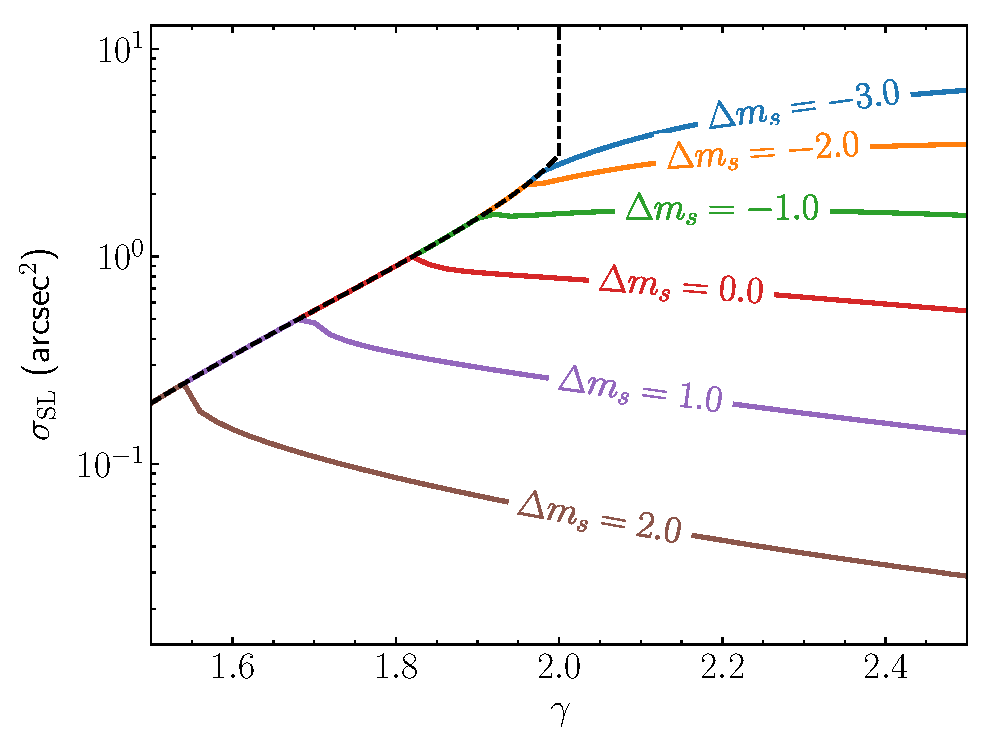
\includegraphics[width=\columnwidth]{axisymm_pl_crosssect.eps}
\caption{
Strong lensing cross-section of an axisymmetric power-law lens and a point source, as a function of the power-law slope $\gamma$.
The system is defined as a strong lens if at least two images are detected.
Different lines correspond to the difference $\Delta m$ between the source magnitude and the survey detection limit for a point source.
The dashed line marks the cross-section in the case in which at least two images are formed, regardless of their magnification.
}
\end{figure}

\subsection{Elliptical lenses, point sources}

\subsection{Elliptical lenses, extended sources}

%__________________________________________________________________

\section{Lens populations simulations}\label{sect:lenspop}


%__________________________________________________________________

\section{Results}\label{sect:results}

There are results.

%__________________________________________________________________

\section{Discussion}\label{sect:discuss}

We discuss.

%__________________________________________________________________

\section{Conclusions}\label{sect:concl}

We conclude.

%\begin{acknowledgements}

%\end{acknowledgements}


\bibliographystyle{aa}
\bibliography{references}

\end{document}


